\documentclass[a4paper,12pt]{article}

\usepackage[english, russian]{babel}
\usepackage[utf8]{inputenc}
\usepackage{graphicx}
\usepackage{subfigure}
%\usepackage{subcaption}
\usepackage{subfig}
\usepackage{amsmath}
\usepackage{listings}
\usepackage[top=2cm, bottom=1.5cm, left=2cm, right=1.5cm]{geometry}
\usepackage{mathtools}
\usepackage[numbered,framed]{matlab-prettifier}
\usepackage{filecontents}
\usepackage[T1]{fontenc}
\usepackage{listings,chngcntr}
\usepackage{float}

\graphicspath{Screen/}

\begin{document}
%\counterwithin{lstlisting}{}
\thispagestyle{empty} %чтобы не было номера на первой странице

\begin{centering}
\textbf{
{\large МИНОБРНАУКИ РОССИИ\\
САНКТ-ПЕТЕРБУРГСКИЙ ГОСУДАРСТВЕННЫЙ\\
ЭЛЕКТРОТЕХНИЧЕСКИЙ УНИВЕРСИТЕТ\\
«ЛЭТИ» ИМ. В.И. УЛЬЯНОВА (ЛЕНИНА)\\
Кафедра САПР}\\
}
\end{centering}


\vspace{7cm}

\begin{centering}
\textbf{{\large 
ОТЧЁТ\\
по лабораторной работе №2\\
по дисциплне \guillemotleft Cети ЭВМ\guillemotright\\
Тема: \guillemotleft Механизмы доступа к узлам сети.\guillemotright\\
}}
\end{centering}

\vspace{4cm}

\begin{tabular}{l c r}
    \textbf{{\large Студенты:}}& \rule{4cm}{1pt} & \textbf{{\large Литвинов К.Л.}}\\
    \textbf{}& \rule{4cm}{1pt} &\textbf{{\large Гарцев Е.А.}}\\
    \textbf{{\large Преподаватель:}}& \hspace{2cm} \rule{4cm}{1pt} \hspace{2cm} & \textbf{{\large Горячев А.В.}}\\
\end{tabular}

\vspace{6cm}


\begin{centering}
	{\large
Санкт-Петербург \\
2020 \\
}
\end{centering}
\newpage
В самом начале была произведена изначальная настройка виртуальных машин в соответствии с
пунктами лабораторной 1-8\\

Далее проверяем доступность нашего сервера:
\begin{figure}[H]
    \center{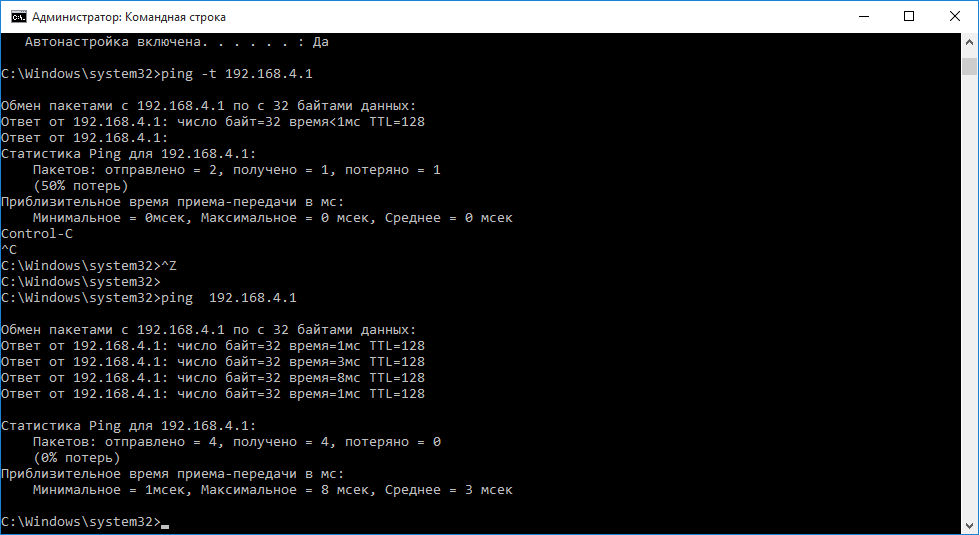
\includegraphics[scale=0.4]{Screen/request2.png}}
\end{figure}
В данном случае нам удаётся связаться с нашим сервером.\\
Теперь попытаемся свзяатся с сервером соседа:
\begin{figure}[H]
    \center{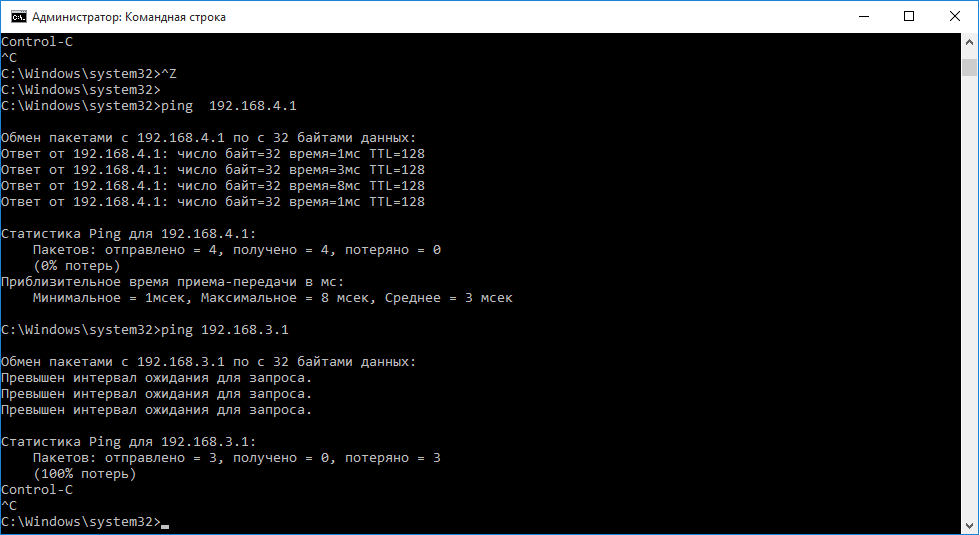
\includegraphics[scale=0.4]{Screen/request3.png}}
\end{figure}
В данном случае нам не удаётся связатся с сервером.\\
В заключении попытаемся связатся с сервером коллег через наш сервер:
\begin{figure}[H]
    \center{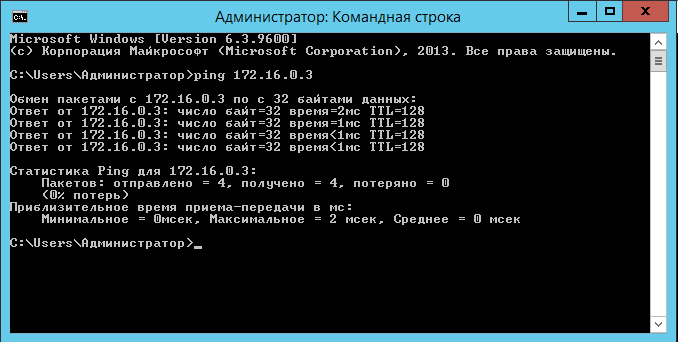
\includegraphics[scale=0.4]{Screen/request4.png}}
\end{figure}
В этой ситуации у нас получается обратится к соседнему серверу.

\section*{Вывод}

После проделанных действий мы видим, что связь между машинами происходит только тогда, 
когда они в одной сети. Получилось, что успешное взаимодействие было только между сервером и
рабочей станции, находившимся на одном компьютере (через внутреннюю сеть) и двумя серверами, 
запущенными на разных компьютерах (через сеть учебного класса).
\end{document}